% Adapted from figures/swat/SWAT_ICS_Architecture.pdf.
% Scientific source: Goh et al., Sections 2 and 4, Figures 2-3 and Table 2.
% Use SWaT's two network levels; omit unsupported cloud/IT annotations.
\documentclass[border=1pt]{standalone}
% Shared typography and palette for the three corrected SWaT context figures.
% Geometry is in millimetres; 140 mm fits the thesis text block at native scale.
\usepackage[T1]{fontenc}
\usepackage{tgheros}
\renewcommand{\familydefault}{\sfdefault}
\usepackage{tikz}
\usetikzlibrary{calc,patterns}
\definecolor{swatblue}{HTML}{0065BD}
\definecolor{swatlight}{HTML}{98C6EA}
\definecolor{swatgrey}{HTML}{666666}
\tikzset{every node/.style={font=\fontsize{8}{10}\selectfont},
  panel/.style={draw=black!30,fill=white,line width=0.4pt},
  stage/.style={draw=swatblue,fill=swatblue,text=white,align=center,
    minimum height=10mm,text width=19mm,inner sep=0.5mm},
  smalllabel/.style={font=\fontsize{7}{8.5}\selectfont,text=swatgrey}}

\begin{document}
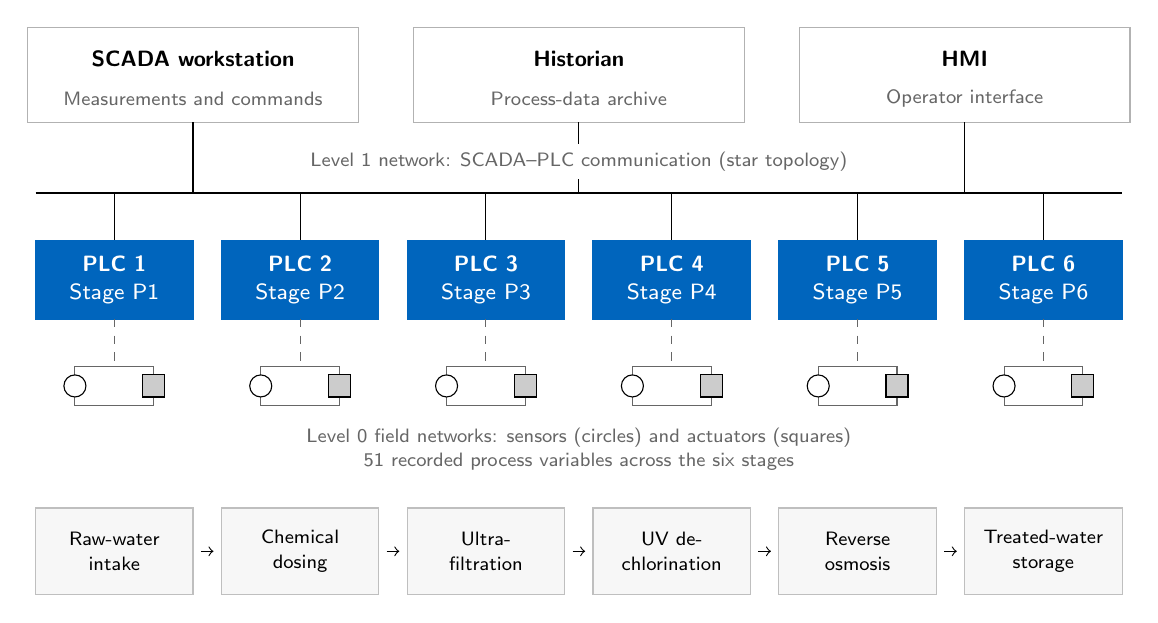
\begin{tikzpicture}[x=1mm,y=1mm]
  \path[use as bounding box] (0,0) rectangle (140,72);
  \foreach \x/\title/\subtitle in {21/SCADA workstation/Measurements and commands,
      70/Historian/Process-data archive,119/HMI/Operator interface} {
    \draw[panel] (\x-21,60) rectangle (\x+21,72);
    \node[font=\bfseries\fontsize{8}{10}\selectfont] at (\x,68) {\title};
    \node[smalllabel] at (\x,63) {\subtitle};
    \draw (\x,60) -- (\x,51);
  }
  \draw[line width=0.7pt] (1,51) -- (139,51);
  \node[fill=white,inner sep=1mm,smalllabel] at (70,55)
    {Level 1 network: SCADA--PLC communication (star topology)};
  \foreach \i/\x in {1/11,2/34.6,3/58.2,4/81.8,5/105.4,6/129} {
    \draw (\x,51) -- (\x,45);
    \node[stage] at (\x,40) {\textbf{PLC \i}\\Stage P\i};
    \draw[dashed,draw=swatgrey] (\x,35) -- (\x,29);
    \draw[draw=swatgrey] (\x-5,24) rectangle (\x+5,29);
    \draw[fill=white] (\x-5,26.5) circle (1.4);
    \draw[fill=black!20] (\x+3.6,25.1) rectangle (\x+6.4,27.9);
  }
  \node[smalllabel,align=center] at (70,18.5)
    {Level 0 field networks: sensors (circles) and actuators (squares)\\
    51 recorded process variables across the six stages};
  \foreach \x/\name in {11/{Raw-water\\intake},34.6/{Chemical\\dosing},
    58.2/{Ultra-\\filtration},81.8/{UV de-\\chlorination},
    105.4/{Reverse\\osmosis},129/{Treated-water\\storage}} {
    \node[draw=black!25,fill=black!3,align=center,text width=19mm,
      minimum height=11mm,inner sep=0.5mm,font=\fontsize{7.5}{9}\selectfont]
      at (\x,5.5) {\name};
  }
  \foreach \x in {22,45.6,69.2,92.8,116.4}
    \draw[->] (\x,5.5) -- (\x+1.6,5.5);
\end{tikzpicture}
\end{document}
